\chapter{Spectroscopy}


%%%%%%%%%%%%%%%%%%%%%%%%%%%%%%%%%%%%%%%%%%%%%%%%%%%%%%%%%
%%%%%%%%%%%%%%%%%%%%%%%%%%%%%%%%%%%%%%%%%%%%%%%%%%%%%%%%%
%%%%%%%%%%%%%%%%%%%%%%%%%%%%%%%%%%%%%%%%%%%%%%%%%%%%%%%%%


%%%%%%%%%%%%%%%%%%%%%%%%%%%%%%%%%%%%%%%%%%%%%%%%%%%%%%%%%
%%%%%%%%%%%%%%%%%%%%%%%%%%%%%%%%%%%%%%%%%%%%%%%%%%%%%%%%%
%%%%%%%%%%%%%%%%%%%%%%%%%%%%%%%%%%%%%%%%%%%%%%%%%%%%%%%%%

\section{Generalized Eigenvalue Problem}\label{app::GEVP}


%%%%%%%%%%%%%%%%%%%%%%%%%%%%%%%%%%%%%%%%%%%%%%%%%%%%%%%%%
%%%%%%%%%%%%%%%%%%%%%%%%%%%%%%%%%%%%%%%%%%%%%%%%%%%%%%%%%
%%%%%%%%%%%%%%%%%%%%%%%%%%%%%%%%%%%%%%%%%%%%%%%%%%%%%%%%%

\subsection{Derivation}
Here we present a derivation of the generalized eigenvalue problem. Considering a basis of operators $\{\mathcal{O}_i\}$ composed of the basic quark and gluon fields of QCD, having the quantum numbers of the desired hadrons, we seek a procedure by which we can maximize the signal to create a hadronic eigenstate of the finite volume Hamiltonian, $\hat{H}$.

Any operator, $\mathcal{O}_i$, acting on the vacuum, $| 0 \rangle $,  effects to create a tower of eigenstates of the Hamiltonian. 
\begin{equation}
\mathcal{O}_i^\dagger | 0 \rangle = \sum_{\estate{n}} \frac{ | \estate{n} \rangle \langle \estate{n} | \mathcal{O}_i^\dagger | 0 \rangle }{2E_{\estate{n}}}  
\end{equation}
Here we are interested only in the lowest lying eigenstates. We will proceed by considering a matrix of two-point functions, $\mathbf{C}$, whose elements are defined:
\begin{equation*}
C_{ij}(t)  \equiv \langle 0 | \mathcal{O}_i(t) \mathcal{O}_j(0) | 0 \rangle = \sum_{\estate{n}} \frac{| \langle \estate{n} | \mathcal{O}_i^\dagger | 0 \rangle |^2}{2E_{\estate{n}}}  e^{-E_{\estate{n}} t}.
\end{equation*}
We have written the spectral representation of the correlation function where we have performed the time evolution $\mathcal{O}(t) = e^{\hat{H}t}\mathcal{O}(0)e^{-\hat{H}t}$, $\hat{H}|\estate{n} \rangle =  E_{\estate{n}}|\estate{n} \rangle$. The vacuum is defined to have zero energy. It is clear that the two point function gives us information about the spectrum of the theory and asymptotically decays to the ground state.

Before continuing we remark that provided our basis of operators is \emph{linearly independent} it also follows that the matrix $\mathbf{C}$ is positive definite which we now prove. Denoting $Z_i^{\estate{n}} \equiv \langle \estate{n} | \mathcal{O}_i^\dagger | 0 \rangle$ ,where we may choose a phasing convention such that all $Z_i^{\estate{n}}$ are real numbers, the $m\times m$ correlation matrix may be decomposed as:

\begin{equation}
\mathbf{C} = \sum_{\estate{n}} \begin{bmatrix} 
g_0^{\estate{n}}g_0^{\estate{n}}  & g_0^{\estate{n}}g_1^{\estate{n}} & \cdots & g_0^{\estate{n}}g_m^{\estate{n}} \\
g_1^{\estate{n}}g_0^{\estate{n}}  & g_1^{\estate{n}}g_1^{\estate{n}} & \cdots & g_1^{\estate{n}}g_m^{\estate{n}} \\
\vdots  					  & 						       & \ddots & \vdots  \\
g_m^{\estate{n}}g_0^{\estate{n}}  & g_m^{\estate{n}}g_1^{\estate{n}} & \cdots & g_m^{\estate{n}}g_m^{\estate{n}} \\
\end{bmatrix}
\end{equation}

where $g_i^{\estate{n}} \equiv \frac{Z_i^{\estate{n}}}{\sqrt{2E_{\estate{n}}}}e^{-E_{\estate{n}}t/2}$. This matrix may then be factorized as 
\begin{equation*}
\mathbf{C} =  \begin{bmatrix} 
g_0^{\estate{0}} & g_0^{\estate{1}} & \cdots &g_0^{\estate{n}} \\
g_1^{\estate{0}} & g_1^{\estate{1}} & \cdots &g_1^{\estate{n}} \\
\vdots &  & \ddots & \vdots \\
g_m^{\estate{0}} & g_m^{\estate{1}} & \cdots &g_m^{\estate{n}} \\
\end{bmatrix} \times 
 \begin{bmatrix} 
g_0^{\estate{0}} & g_1^{\estate{0}} & \cdots &g_m^{\estate{0}} \\
g_0^{\estate{1}} & g_1^{\estate{1}} & \cdots &g_m^{\estate{1}} \\
\vdots &  & \ddots & \vdots \\
g_0^{\estate{n}} & g_1^{\estate{n}} & \cdots &g_m^{\estate{n}} \\
\end{bmatrix} = \mathbf{A}^T\mathbf{A} \label{app::pos_def_decomp}
\end{equation*}

Where the matrix $\mathbf{A}$ is an $N\times m$ \emph{rectangular matrix}. A sufficient condition for a matrix to be positive definite is if the product $z^T M z  >0 $ for any non-null vector, $z$. Then $z^T C z$ = $(\mathbf{A}z)^T (\mathbf{A}z) > 0$. Thus $\mathbf{C}$ is positive definite. In the case that our operators are not linearly independent we must first remove the null-space after which the proof goes through identically.   

Having shown that correlation matrix is positive definite we now turn to the problem at hand, namely, we seek a procedure by which we can maximize
\begin{equation}
\Omega(\vec{\alpha}) \equiv \sum_{ij} \alpha_i \langle 0 | \mathcal{O}_i(t) \mathcal{O}_j(0) | 0 \rangle \alpha_j,
\end{equation} 
 essentially the amplitude of our signal, as a function of the coefficients $\{\alpha_k\}$ which are real parameters. In order to introduce an absolute normalization for the coefficients we also include a Lagrange multiplier.  We then seek to extremize (maximize)  the function 
\begin{equation}
\Lambda( \{\alpha_k\} , \lambda ) = \sum_{ij} \alpha_i \langle 0 | \mathcal{O}_i(t) \mathcal{O}_j(0) | 0 \rangle \alpha_j - \lambda \left( \left[\sum_{ij} \alpha_i \langle 0 | \mathcal{O}_i(t_0) \mathcal{O}_j(0) | 0 \rangle \alpha_j \right] - \mathcal{N} \right)
\end{equation}
where it is understood that $t_0 < t$. This equation may be written more compactly in matrix form as 
\begin{equation*}
\Lambda( \vec{\mathbf{\alpha}} , \lambda) = \vec{\mathbf{\alpha}}^T\cdot \mathbf{C}(t) \cdot \vec{\mathbf{\alpha}} - \lambda \left(  \vec{\mathbf{\alpha}}^T\cdot \mathbf{C}(t_0) \cdot \vec{\mathbf{\alpha}} - \mathcal{N} \right)
\end{equation*} 
where $\vec{\alpha}$ is a column vector and $\mathbf{C}$ is a real, symmetric, and positive definite matrix. We proceed in the standard method by taking the first derivative of the function $\Lambda(\{\alpha_k\} , \lambda)$ and setting it to zero which gives us the locations of the critical points (maxima, minima, and saddle points). 

\begin{align*}
\frac{\partial}{\partial \alpha_k} \Lambda( \vec{\mathbf{\alpha}} , \lambda) = 2 \left( \left[\sum_j  \langle 0 | \mathcal{O}_k(t) \mathcal{O}_j(0) | 0 \rangle \alpha_j\right] - \lambda \left[\sum_j  \langle 0 | \mathcal{O}_k(t_0) \mathcal{O}_j(0) | 0 \rangle \alpha_j\right] \right)  = 0 \\
\frac{\partial}{\partial \lambda} \Lambda( \vec{\mathbf{\alpha}} , \lambda) = \left[\sum_{ij} \alpha_i \langle 0 | \mathcal{O}_i(t_0) \mathcal{O}_j(0) | 0 \rangle \alpha_j \right] - \mathcal{N} = 0
\end{align*}

Re-expressing the above set of equations in matrix form yields 
\begin{align}
\mathbf{C}(t) \cdot \vec{\alpha} = \lambda \mathbf{C}(t_0) \cdot \vec{\alpha} \notag \\ 
\vec{\mathbf{\alpha}}^T\cdot \mathbf{C}(t_0) \cdot \vec{\alpha} = \mathcal{N}.  \label{app::gevp_primitive}
\end{align}

A similar derivation follows when one considers multiple sets of $\{\alpha^{(\estate{n})}_i\}$ and promotes the normalization condition to an orthogonality condition. For a basis of $N$ operators we have access to, at most, $N$ states, each vector $\{\alpha^{(\estate{n})}_i\}$ maping to one low lying eigenstates of the Hamiltonian residing within the reach of our basis. Relabeling Equation \ref{app::gevp_primitive}, $\alpha^{(\estate{n})}_i \rightarrow v^{(\estate{n})}_i$, we arrive at the standard representation of the Generalized Eigenvalue Problem, 
 
\begin{align}
C_{ij}(t)v^{(\estate{n})}_j   = \lambda^{(\estate{n})} C_{ij}(t_0)v^{(\estate{n})}_j \notag \\ 
v^{(\estate{n})}_i C(t_0)_{ij}v^{(\estate{m})}_j  = \delta_{\estate{n}\estate{m}}.  \label{app::gevp}
\end{align}

%%%%%%%%%%%%%%%%%%%%%%%%%%%%%%%%%%%%%%%%%%%%%%%%%%%%%%%%%
%%%%%%%%%%%%%%%%%%%%%%%%%%%%%%%%%%%%%%%%%%%%%%%%%%%%%%%%%
%%%%%%%%%%%%%%%%%%%%%%%%%%%%%%%%%%%%%%%%%%%%%%%%%%%%%%%%%

\subsection{Implementation}
The variational method involves solving the generalized eigenvalue problem 
\begin{equation}
C_{ij}(t)v^{(\estate{n})}_j   = \lambda^{(\estate{n})} C_{ij}(t_0)v^{(\estate{n})}_j. \label{eqn:gen_eig}
\end{equation}
This can be achieved via reformulating the problem as a standard eigenvalue problem. In practice we choose to do this via Singular Value Decomposition.  It is well known that any matrix $M$, real or complex, may be factorized to the form $M = U\Sigma V^{\dagger}$, where $U$ and $V$ are unitary matrices and $\Sigma$ is a diagonal matrix whose entries are the ``singular values'' of $M$. In the case of a symmetric  matrix it is evident that $M = U\Sigma U^T$. It also follows that algebraically $M^{-1} = V\cdot [\mathrm{diag}(1/\sigma_j)]\cdot U^T$, for $\sigma_j$ the j$^{\text{th}}$ singular value of $\Sigma$.  Further in the event that one of the $\sigma_j$'s is singular or near singular, it can be shown that the best approximation to the inverse, the pseudoinverse (Moore-Penrose Inverse), is obtained by setting $\frac{1}{\sigma_j} \rightarrow 0$. This machinery will be useful in constructing a solution involving SVD below.
\par
Noting Equation \ref{eqn:gen_eig} again,
\begin{equation*}
C(t)V(t) = C(t_0)V(t)\Lambda(t).
\end{equation*}
We see we can decompose $C(t_0) = U(t_0)\Sigma(t_0)U^T(t_0)$ and the above becomes
\begin{equation*}
C(t)V(t) = U(t_0)\Sigma(t_0)U^T(t_0)V(t)\Lambda(t).
\end{equation*}
Multiplying from the left by $\frac{1}{\sqrt{\Sigma^{+}}}U^T$, where $\frac{1}{\sqrt{\Sigma^{+}}}$ is the square root of the pseudoinverse ($\Sigma$ is diagonal so the inverse square root is trivial) of the singular value matrix with singular values reset to 0, we see the above becomes
\begin{equation*}
\frac{1}{\sqrt{\Sigma^{+}}}U^TC(t)V(t) = \sqrt{\Sigma^{+}}U^TV(t)\Lambda(t)
\end{equation*}
Where we have used the property $U^TU = \mathbb{1}$.  Now inserting $\mathbb{1} = U\sqrt{\frac{\Sigma^{+}}{\Sigma^{+}}}U^T$ we see we can recover a standard eigenvalue problem,
\begin{align*}
\label{eqn:svd_gen_eig}
\left[\frac{1}{\sqrt{\Sigma^{+}}}U^TC(t)U\frac{1}{\sqrt{\Sigma^{+}}}\right] \left[\sqrt{\Sigma^{+}}U^TV(t)\right] &= \left[\sqrt{\Sigma^{+}}U^TV(t)\right]\Lambda(t).
\end{align*}
Which with the identification of $M = \frac{1}{\sqrt{\Sigma^{+}}}U^TC(t)U\frac{1}{\sqrt{\Sigma^{+}}}$ and $W(t) = \sqrt{\Sigma^{+}}U^TV(t)$, forms a standard eigensystem, $M W(t) = W(t)\Lambda(t)$. The generalized eigenvectors are recoverable from the standard eigenvectors by simple matrix algebra, $V(t) = U\frac{1}{\sqrt{\Sigma^{+}}}W(t)$. 

In explicit calculation the correlation functions we compute are statistical approximations and as such we have some noise or variance associated with each element of the matrix $C(t)$. It is possible for the noise to combine in such a way as to introduce an approximate null-space into the correlation matrices, an approximate linear dependence within the basis arising from the variance associated with each element. SVD provides, via pseudoinversion, a method by which we can eliminate this null space. We show a toy example of the removal of null space in \figref{fig::SVDProjGraphic}.

\afterpage{
\begin{figure}[htbp]
\begin{centering}
  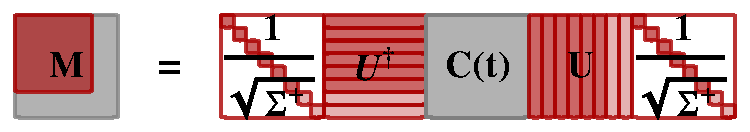
\includegraphics[width=0.8\linewidth]{figures/ProjectionGraphicFinal.pdf}
  \caption{ A toy example of SVD resetting. The gray box is the full rank matrix while $M$ represents the subspace we wish to eigendecompose. The transparent column and elements represent the portion of the full rank matrix that was approximately null which we remove via SVD resetting. \label{fig::SVDProjGraphic}}
    \end{centering}
\end{figure}
\clearpage
}


%%%%%%%%%%%%%%%%%%%%%%%%%%%%%%%%%%%%%%%%%%%%%%%%
%%% MOMENTUM CONSERVATION
%%%%%%%%%%%%%%%%%%%%%%%%%%%%%%%%%%%%%%%%%%%%%%%%

\section{Momentum conservation in a finite-volume}\label{app::two-point}

We define meson eigenstates which in infinite volume have normalization
\begin{equation}
 \big\langle \mathfrak{n}(\vec{k}) \big| \mathfrak{n}'(\vec{p}) \big\rangle = \delta_{\mathfrak{n}\mathfrak{n}'}(2\pi)^3 \, 2 E_{\vec{k}} \; \delta^{(3)}( \vec{k} - \vec{p} \,),
\end{equation}
such that the completeness relation takes the form
\begin{equation}
1 = \sum_\mathfrak{n} \int \!\! \frac{d^3 \vec{k} }{(2\pi)^3} \, \frac{1}{2  E_{\mathfrak{n}}(\vec{k})  } 
	\big| \mathfrak{n}(\vec{k}) \big\rangle \big\langle \mathfrak{n}(\vec{k}) \big|.
\end{equation}
In a periodic cubic volume, $L \times L \times L$, the allowed momenta of free particles is quantized, $\vec{k} = \tfrac{2\pi}{L} \vec{n}_k$, where $\vec{n}_k = \big(n_x, n_y, n_z \big)$ and the completeness relation becomes
\begin{equation}
1 = \frac{1}{L^3} \sum_\mathfrak{n} \sum_{\vec{n}_k} \, \frac{1}{2 E_{\mathfrak{n}}(\vec{k}) } 
	\big| \mathfrak{n}(\vec{k}) \big\rangle \big\langle \mathfrak{n}(\vec{k}) \big|. \label{completeness}
\end{equation}


Two-point correlation functions in which the source and sink operators are projected into definite momentum have a spectral representation which can be obtained by inserting Eq.~\ref{completeness},

\begin{align*}
C(t) 	&= \big\langle 0 \big| \mathcal{O}^{\,}_\mathrm{f}(\vec{p}_{\mathrm{f}}, t) \, \mathcal{O}^\dag_\mathrm{i}(\vec{p}_\mathrm{i}, 0) \big| 0 \big\rangle \\ 
		&= \big\langle 0 \big| \sum\nolimits_{\vec{x}} e^{i \vec{p}_\mathrm{f}\cdot \vec{x} }\,  \mathcal{O}^{\,}_\mathrm{f}(\vec{x}, t)\, 
		\sum\nolimits_{\vec{y}} e^{-i \vec{p}_\mathrm{i}\cdot \vec{y} }\,  \mathcal{O}^{\dag}_\mathrm{i}(\vec{y}, 0) \big| 0 \big\rangle \\
		&= \frac{1}{L^3} \sum_\mathfrak{n} \sum_{\vec{n}_k} \, \frac{1}{2 E_\mathfrak{n}(\vec{k}) } 
		\,\big( L^3 \delta_{\vec{p}_\mathrm{f} \vec{k}} \,\big)
		\,\big( L^3 \delta_{\vec{p}_\mathrm{i} \vec{k}} \,\big) 
		e^{-E_{\mathfrak{n}} t} \; 
		\big\langle 0 \big| \mathcal{O}_\mathrm{f}(\vec{x}=\vec{0}, 0) \big| \mathfrak{n}(\vec{k}) \big\rangle
		\big\langle \mathfrak{n}(\vec{k}) \big| \mathcal{O}^\dag_\mathrm{i}(\vec{y}=\vec{0}, 0) \big| 0\big\rangle \\
		&= L^3 \delta_{\vec{p}_\mathrm{f} , \vec{p}_\mathfrak{i}} \sum_\mathfrak{n} \frac{1}{2 E_\mathfrak{n} } 
		e^{-E_{\mathfrak{n}} t} \; 
		\big\langle 0 \big| \mathcal{O}_\mathrm{f}(\vec{0}, 0) \big| \mathfrak{n}(\vec{p}_\mathrm{i}) \big\rangle
		\big\langle \mathfrak{n}(\vec{p}_\mathrm{i}) \big| \mathcal{O}^\dag_\mathrm{i}(\vec{0}, 0) \big| 0\big\rangle,
\end{align*}
where we note an explicit factor of the lattice volume, $L^3$. 

Three-point correlation functions projected into definite source, sink and current momentum have a spectra representation,
\begin{align*}
C(t) 	&= 	\big\langle 0 \big| \mathcal{O}^{\,}_\mathrm{f}(\vec{p}_\mathrm{f}, t_\mathrm{f}) \,
			j(\vec{q}, t) \, 
			\mathcal{O}^\dag_\mathrm{i}(\vec{p}_\mathrm{i}, t_\mathrm{i}) \big| 0 \big\rangle \\
		&= \big\langle 0 \big| \sum\nolimits_{\vec{x}} e^{i \vec{p}_\mathrm{f}\cdot \vec{x} }\, \mathcal{O}^{\,}_\mathrm{f}(\vec{x}, t_\mathrm{f})\, 
		\sum\nolimits_{\vec{z}} e^{-i \vec{q} \cdot \vec{z} }\, j(\vec{z}, t)\,
		\sum\nolimits_{\vec{y}} e^{-i \vec{p}_\mathrm{i}\cdot \vec{y} }\, \mathcal{O}^{\dag}_\mathrm{i}(\vec{y}, t_\mathrm{i}) \big| 0 \big\rangle \\ 
		&= L^3 \delta_{\vec{p}_\mathrm{f} , \vec{p}_\mathfrak{i}+\vec{q}} \sum_{\mathfrak{n}_\mathrm{i},\mathfrak{n}_\mathrm{f} } \frac{1}{2 E_{\mathfrak{n}_\mathrm{i}} }\frac{1}{2 E_{\mathfrak{n}_\mathrm{f}} } 
		e^{-E_{\mathfrak{n}_\mathrm{f}} (t_f - t)} e^{-E_{\mathfrak{n}_\mathrm{i}} (t - t_i)} \;  
\\
		&\qquad\qquad\qquad\times\big\langle 0 \big| \mathcal{O}_\mathrm{f}(\vec{0}, 0) \big| \mathfrak{n}_\mathrm{f}(\vec{p}_\mathrm{f}) \big\rangle
		\big\langle \mathfrak{n}_\mathrm{f}(\vec{p}_\mathrm{f}) \big| j(\vec{0},0) \big| \mathfrak{n}_\mathrm{i}(\vec{p}_\mathrm{i}) \big\rangle
		\big\langle \mathfrak{n}_\mathrm{i}(\vec{p}_\mathrm{i}) \big| \mathcal{O}^\dag_\mathrm{i}(\vec{0}, 0) \big| 0\big\rangle,	
\end{align*}
which again features an explicit factor of the lattice volume, $L^3$. This volume factor, common to two-point and three-point functions may conventionally be absorbed into the meson creation/annihilation matrix elements.




%%%%%%%%%%%%%%%%%%%%%%%%%%%%%%%%%%%%%%%%%%%%%%%%%%%%%%%%%
%%%%%%%%%%%%%%%%%%%%%%%%%%%%%%%%%%%%%%%%%%%%%%%%%%%%%%%%%
%%%%%%%%%%%%%%%%%%%%%%%%%%%%%%%%%%%%%%%%%%%%%%%%%%%%%%%%%

\section{Subduction Coefficients for Mesons in Flight }\label{app::Subduce}

 
\begin{table}
\begin{centering}
\begin{tabular}{c|c|c|c}
\textbf{Group} & $|\lambda|^{\tilde{\eta}}$ & \textbf{$\Lambda(\mu)$} & \textbf{$\mathcal{S}_{\Lambda,\mu}^{\tilde{\eta},\lambda}$} \\
\hline
$\Dic_{4}$ 
 & $0^+$ & $A_1(1)$ & $1$ \\
$(n,0,0)$
 & $0^-$ & $A_2(1)$ & $1$ \\
 & $1$   & $E_2\left(\begin{smallmatrix}1 \\ 2\end{smallmatrix}\right)$ & $(\delta_{s,+} \pm \tilde{\eta} \delta_{s,-})/\sqrt{2}$ \\
 & $2$   & $B_1(1)$ & $(\delta_{s,+} + \tilde{\eta} \delta_{s,-})/\sqrt{2}$ \\
 & $2$   & $B_2(1)$ & $(\delta_{s,+} - \tilde{\eta} \delta_{s,-})/\sqrt{2}$ \\
 & $3$   & $E_2\left(\begin{smallmatrix}1 \\ 2\end{smallmatrix}\right)$ & $(\pm\delta_{s,+} + \tilde{\eta} \delta_{s,-})/\sqrt{2}$ \\
 & $4$   & $A_1(1)$ & $(\delta_{s,+} + \tilde{\eta} \delta_{s,-})/\sqrt{2}$ \\
 & $4$   & $A_2(1)$ & $(\delta_{s,+} - \tilde{\eta} \delta_{s,-})/\sqrt{2}$ \\
\hline
$\Dic_{2}$
 & $0^+$ & $A_1(1)$ & $1$ \\
$(n,n,0)$
 & $0^-$ & $A_2(1)$ & $1$ \\
 & $1$   & $B_1(1)$ & $(\delta_{s,+} + \tilde{\eta} \delta_{s,-})/\sqrt{2}$ \\
 & $1$   & $B_2(1)$ & $(\delta_{s,+} - \tilde{\eta} \delta_{s,-})/\sqrt{2}$ \\
 & $2$   & $A_1(1)$ & $(\delta_{s,+} + \tilde{\eta} \delta_{s,-})/\sqrt{2}$ \\
 & $2$   & $A_2(1)$ & $(\delta_{s,+} - \tilde{\eta} \delta_{s,-})/\sqrt{2}$ \\
 & $3$   & $B_1(1)$ & $(\delta_{s,+} + \tilde{\eta} \delta_{s,-})/\sqrt{2}$ \\
 & $3$   & $B_2(1)$ & $(\delta_{s,+} - \tilde{\eta} \delta_{s,-})/\sqrt{2}$ \\
 & $4$   & $A_1(1)$ & $(\delta_{s,+} + \tilde{\eta} \delta_{s,-})/\sqrt{2}$ \\
 & $4$   & $A_2(1)$ & $(\delta_{s,+} - \tilde{\eta} \delta_{s,-})/\sqrt{2}$ \\
\hline
$\Dic_{3}$
 & $0^+$ & $A_1(1)$ & $1$ \\
$(n,n,n)$
 & $0^-$ & $A_2(1)$ & $1$ \\
 & $1$   & $E_2\left(\begin{smallmatrix}1 \\ 2\end{smallmatrix}\right)$ & $(\delta_{s,+} \pm \tilde{\eta} \delta_{s,-})/\sqrt{2}$ \\
 & $2$   & $E_2\left(\begin{smallmatrix}1 \\ 2\end{smallmatrix}\right)$ & $(\pm\delta_{s,+} - \tilde{\eta} \delta_{s,-})/\sqrt{2}$ \\
 & $3$   & $A_1(1)$ & $(\delta_{s,+} - \tilde{\eta} \delta_{s,-})/\sqrt{2}$ \\
 & $3$   & $A_2(1)$ & $(\delta_{s,+} + \tilde{\eta} \delta_{s,-})/\sqrt{2}$ \\
 & $4$   & $E_2\left(\begin{smallmatrix}1 \\ 2\end{smallmatrix}\right)$ & $(\delta_{s,+} \mp \tilde{\eta} \delta_{s,-})/\sqrt{2}$ \\
\hline
\end{tabular}
\caption{Subduction coefficients, $\mathcal{S}_{\Lambda,\mu}^{\tilde{\eta},\lambda}$, for $|\lambda| \leq 4$ with $s \equiv \text{sign}(\lambda)$. Here $\tilde{\eta} \equiv P(-1)^J$ with $J$ and $P$ the spin and parity of the operator $\mathbb{O}^{J,P,\lambda}(\vec{p}=\vec{0})$.  The subduced helicity operators are different orthogonal combinations of the two signs of helicity, $+|\lambda|$ and $-|\lambda|$. }
\label{tab::subductions}
\end{centering}
\end{table} 

\clearpage







